\chapter{System Design} \label{chap:design}

System design is the process of defining the architecture, components, modules, interfaces, and data schemas for a software system to satisfy specified operational and academic requirements. This chapter presents the comprehensive architectural and detailed engineering design of \textbf{RecruitSense}, an intelligent, trust-oriented Applicant Tracking System (ATS) and Automated Resume Screening Platform.

The core design objective of RecruitSense is not merely to store candidate applications, but to actively eliminate operational ambiguity and recruitment bottlenecks by introducing decoupled microservices, controlled hiring pipeline state transitions, explainable AI-driven candidate screening, role-governed administration, and auditable data flows. Each architectural decision was guided by the principle that algorithmic transparency, data security, and sub-second operational responsiveness must be first-class system concerns.

\section{System Architecture}
RecruitSense follows a layered, decoupled service-oriented architecture comprising four primary tiers: the Presentation Tier (React SPA Client), the Business Application Tier (Laravel REST API), the Computational AI/ML Inference Tier (Python Flask Microservice), and the Persistence and Identity Tier (MySQL 8.0 Relational Database and Secure File Storage) \cite{fielding2000rest}. Each layer maintains strictly defined operational boundaries and communicates over standard RESTful HTTP protocols with JSON payloads.

\begin{figure}[h!]
\centering
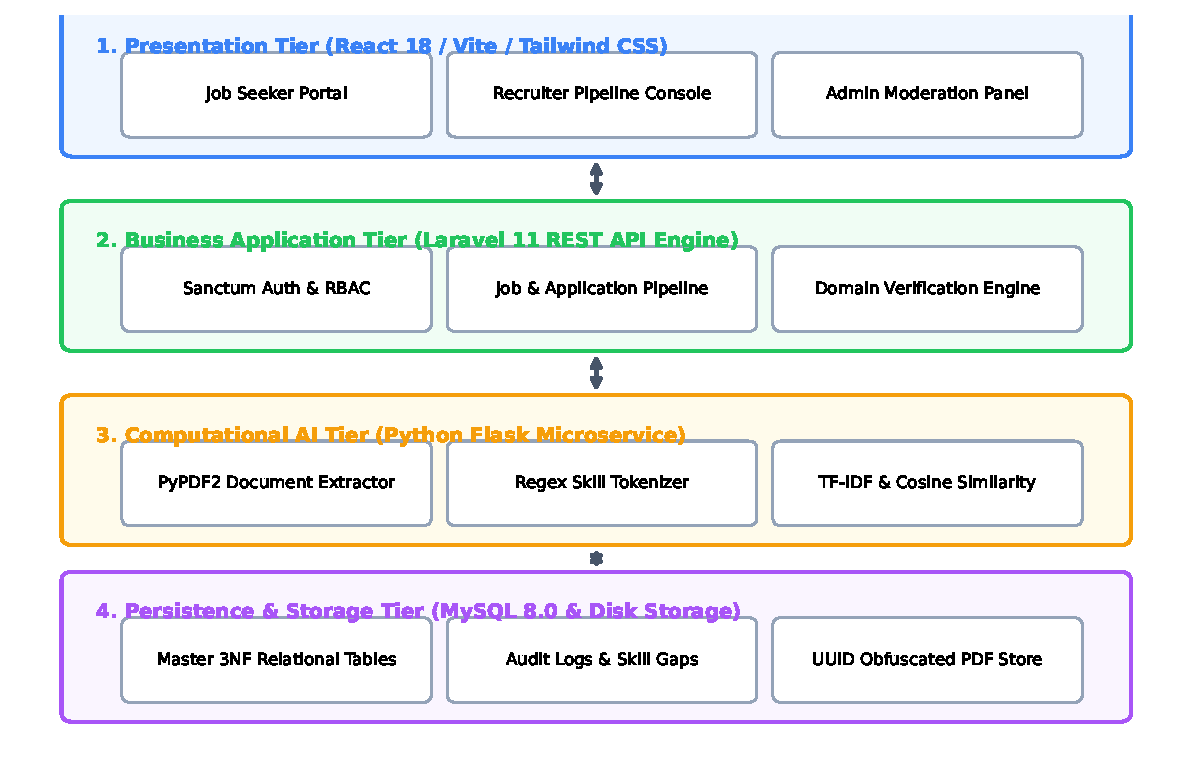
\includegraphics[width=0.9\linewidth]{figures/sys_architecture.pdf}
\caption{Decoupled Multi-Tier System Architecture of RecruitSense}
\label{fig:sys_arch_detail}
\end{figure}

\subsection{Frontend Layer (Client SPA)}
The presentation tier is implemented as a Single Page Application using React 18, Vite, and Tailwind CSS. The web client utilizes client-side routing via \texttt{react-router-dom} to deliver instant, fluid transitions without full-page browser refreshes. It serves three distinct user surfaces:
\begin{itemize}
    \item \textbf{Public Job Discovery Surface:} Accessible to all visitors for browsing active job openings, searching technical keywords, and filtering by location, department, or salary without requiring authentication.
    \item \textbf{Authenticated Job Seeker Surface:} Enables candidates to manage profile information, upload PDF resumes, submit applications with real-time feedback, view granular ATS match scores with skill gap visualizers, bookmark jobs, and communicate with recruiters.
    \item \textbf{Recruiter & Admin Surface:} Provides corporate employers with job vacancy creation tools, candidate ranking tables sorted by computed ATS score, stage-by-stage pipeline management, and interview scheduling. Platform administrators access domain verification queues, content moderation tools, and global platform analytics.
\end{itemize}

\subsection{Backend Application Layer}
The backend service layer is developed on Laravel 11 (PHP 8.2+). It serves as the authoritative gateway for business logic, transactional integrity, and security policy enforcement. 

Core responsibilities include:
\begin{itemize}
    \item Authentication and token issuance via Laravel Sanctum.
    \item Role-Based Access Control (RBAC) middleware enforcing least-privilege route access.
    \item Corporate domain validation (\texttt{TrustedEmailDomain}) preventing unverified employer registrations.
    \item Hiring pipeline lifecycle management (\textit{Applied} $\rightarrow$ \textit{Screening} $\rightarrow$ \textit{Shortlisted} $\rightarrow$ \textit{Interview} $\rightarrow$ \textit{Offer} $\rightarrow$ \textit{Rejected}).
    \item Asynchronous file ingestion and orchestration with the Python Flask AI microservice.
\end{itemize}

\subsection{AI/ML Screening Layer}
The artificial intelligence inference layer operates as an independent Python Flask microservice. Separating the AI layer from the transactional API backend isolates CPU-intensive text parsing and matrix algebra from blocking user-facing web requests.

AI capabilities implemented in RecruitSense include:
\begin{itemize}
    \item \textbf{PDF Document Text Extraction:} Reads binary PDF streams page-by-page, strips binary encoding artifacts, and cleans raw text.
    \item \textbf{Boundary-Delimited Skill Extraction:} Matches candidate resume text against an extensive multi-domain technology taxonomy.
    \item \textbf{TF-IDF Cosine Similarity Matching:} Constructs joint vector space models between normalized resumes and job descriptions, computing mathematical similarity percentages.
    \item \textbf{Skill Gap Identification:} Generates structured JSON arrays of matched skills, missing skill gaps, and bonus skills.
\end{itemize}

\subsection{Data and Identity Layer}
Persistent storage is managed through a normalized MySQL 8.0 relational database schema, with candidate resume documents stored securely on encrypted disk storage outside the public web root.

Key data layer features include:
\begin{itemize}
    \item Strict third normal form (3NF) relational design with foreign key cascade constraints.
    \item Eloquent ORM parameterized query binding neutralizing SQL injection risks.
    \item Dedicated tables for users, companies, job seekers, vacancies, applications, skill gaps, messages, and admin settings.
    \item Storage obfuscation renaming uploaded resumes using randomized SHA-256 UUIDs.
\end{itemize}

\subsection{Architectural Rationale}
The architectural design of RecruitSense is justified by five fundamental rationales:
\begin{enumerate}
    \item \textbf{Security-First State Control:} All candidate state transitions, role authorizations, and domain validations are strictly owned and executed on the backend server.
    \item \textbf{Independent Scalability:} The React client, Laravel API, and Flask AI microservice can scale horizontally on distinct compute nodes according to traffic demand.
    \item \textbf{Explainable Trust Design:} Unlike legacy black-box ATS engines, RecruitSense exposes transparent score formulations and color-coded skill gap badges.
    \item \textbf{High Operational Maintainability:} Modular boundaries ensure that changes to AI models or frontend components do not destabilize core database transactions.
    \item \textbf{Lightweight Self-Contained Deployment:} By utilizing Scikit-learn and regex tokenization rather than heavy external paid LLM APIs, the system operates deterministically with zero marginal API cost.
\end{enumerate}

\section{Design Constraints and Assumptions}
The architecture and implementation of RecruitSense were shaped by specific technical, security, and operational constraints.

\subsection{Technical Constraints}
\begin{itemize}
    \item \textbf{AI Inference Latency:} End-to-end PDF parsing and similarity scoring must complete within $2.5\text{ seconds}$ to maintain high responsiveness for applicants.
    \item \textbf{Document Upload Size Limits:} Resumes are capped at a maximum file size of $5\text{MB}$ to prevent server memory exhaustion.
    \item \textbf{CORS and Origin Isolation:} Frontend and backend services operate across different ports during development, requiring strict Cross-Origin Resource Sharing (CORS) origin validation.
    \item \textbf{Deterministic State Transitions:} Application pipeline states are guarded to prevent illegal jumps (e.g., an application cannot transition directly from \textit{Applied} to \textit{Offer Extended} without passing through review).
\end{itemize}

\subsection{Data Constraints}
\begin{itemize}
    \item \textbf{Input Data Quality:} Automated ATS scoring depends on the presence of extractable digital text layers in candidate PDF resumes.
    \item \textbf{Schema Normalization:} Foreign keys enforce referential integrity; deleting an employer profile cleanly cascades to associated job postings and application records.
    \item \textbf{Search Term Normalization:} Query strings are sanitized and case-folded to enable flexible partial matching across job titles and skill tags.
\end{itemize}

\subsection{Security and Compliance Constraints}
\begin{itemize}
    \item \textbf{Least-Privilege RBAC:} User actions are strictly constrained by role middleware (\texttt{'job\_seeker'}, \texttt{'company'}, \texttt{'admin'}).
    \item \textbf{Password Encryption:} Passwords are encrypted using Bcrypt with a work factor of 12 rounds.
    \item \textbf{Resume Document Privacy:} Candidate resumes are stored in access-controlled disk directories and served only through authenticated controller streams.
    \item \textbf{Audit Logging:} Privileged administrative actions (domain approvals, account suspensions) produce durable audit log entries.
\end{itemize}

\subsection{Assumptions}
\begin{itemize}
    \item Users possess basic digital literacy to navigate web forms and upload PDF documents.
    \item Job seekers submit authentic curriculum vitae in standard digital formats (PDF/DOCX).
    \item Corporate recruiters provide representative job descriptions and explicit required skill lists.
\end{itemize}

\section{Design Methodology}
RecruitSense was designed using an **Agile Iterative Framework** combined with **Object-Oriented Analysis and Design (OOAD)** and **Finite State Machine (FSM)** modeling for critical workflows \cite{sommerville2016software}.

\subsection{Incremental Domain Milestones}
Development proceeded across five distinct functional milestones:
\begin{enumerate}
    \item Master relational schema modeling, database migrations, and Sanctum token authentication.
    \item Job vacancy management, multi-role web dashboards, and corporate domain verification.
    \item AI microservice development, PDF text extraction, and TF-IDF similarity algorithms.
    \item Full-stack integration, ATS score visualization, and skill gap badge diagnostics.
    \item System testing, performance benchmarking, and security evaluation.
\end{enumerate}

\subsection{State-Machine Methodology for Hiring Pipelines}
The candidate application lifecycle is modeled as a formal Finite State Machine (FSM) with validated transition rules, as illustrated in Figure \ref{fig:fsm_pipeline}.

\begin{figure}[h!]
\centering
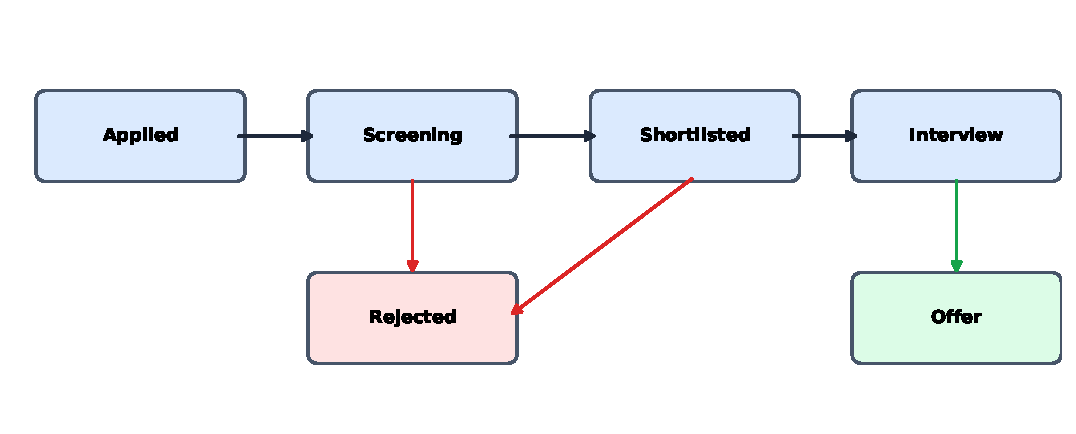
\includegraphics[width=0.8\linewidth]{figures/hiring_fsm.pdf}
\caption{Finite State Machine for Candidate Hiring Pipeline}
\label{fig:fsm_pipeline}
\end{figure}

\section{High-Level Block Diagram}
RecruitSense is structured into four primary operational blocks coordinating across system boundaries:
\begin{enumerate}
    \item \textbf{Presentation Block (React 18 / Tailwind):} Renders responsive client interfaces for Job Seekers, Employers, and Admins.
    \item \textbf{Application Block (Laravel 11 REST API):} Enforces business logic, authentication guards, and database transactions.
    \item \textbf{Intelligence Block (Python Flask AI):} Executes PDF stream text extraction, regex skill tokenization, and TF-IDF cosine similarity scoring.
    \item \textbf{Data Block (MySQL 8.0 & File Storage):} Persists relational tables and access-controlled resume documents.
\end{enumerate}

\begin{figure}[h!]
\centering
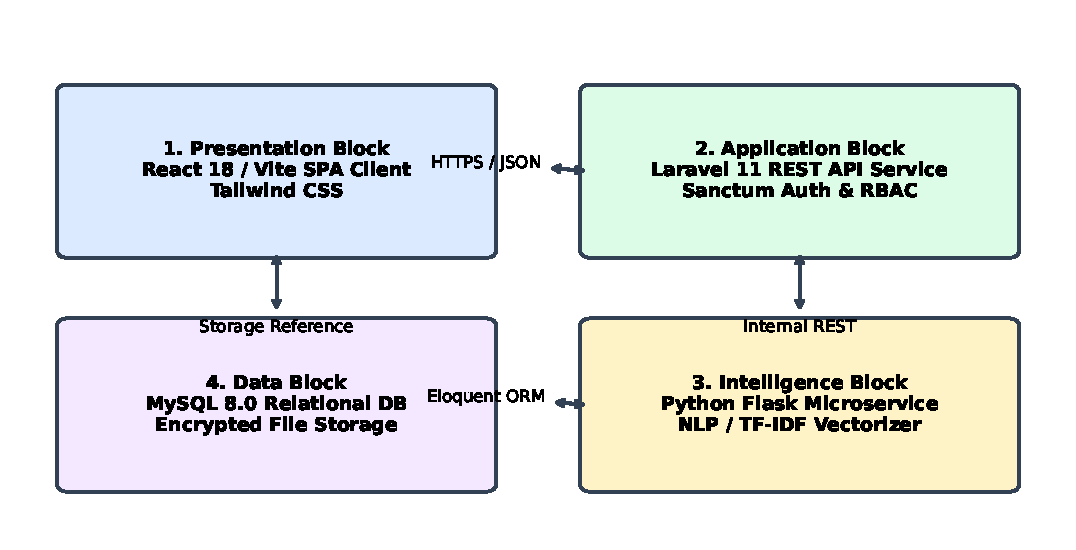
\includegraphics[width=0.8\linewidth]{figures/block_diagram.pdf}
\caption{High-Level Functional Block Diagram of RecruitSense}
\label{fig:high_level_blocks}
\end{figure}

\section{Low-Level Design: System Sequence Diagrams (SSDs)}
This section details the System Sequence Diagrams (SSDs) for the core use cases of RecruitSense, mapping the precise order of message exchanges, payload transfers, and state transitions between actors and subsystems.

\subsection{SSD-01: Browse and Filter Jobs}
As illustrated in Figure \ref{fig:ssd01}, a visitor or registered job seeker searches and filters active job listings on the web portal.

\begin{figure}[h!]
\centering
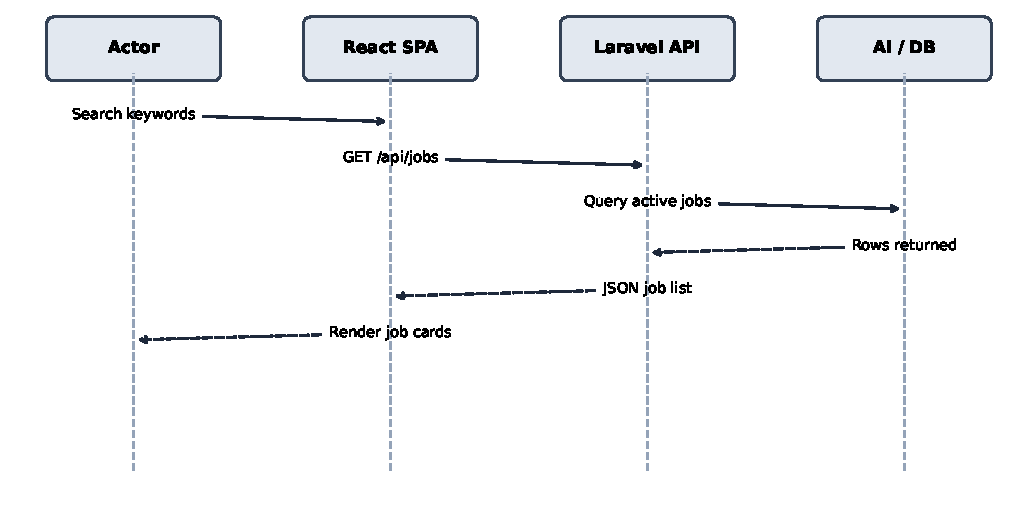
\includegraphics[width=0.75\linewidth]{figures/ssd_01.pdf}
\caption{SSD-01: Browse and Filter Jobs Sequence Diagram}
\label{fig:ssd01}
\end{figure}

\subsection{SSD-02: Register User with Role Assignment}
As shown in Figure \ref{fig:ssd02}, a new user registers with role selection and corporate domain validation.

\begin{figure}[h!]
\centering
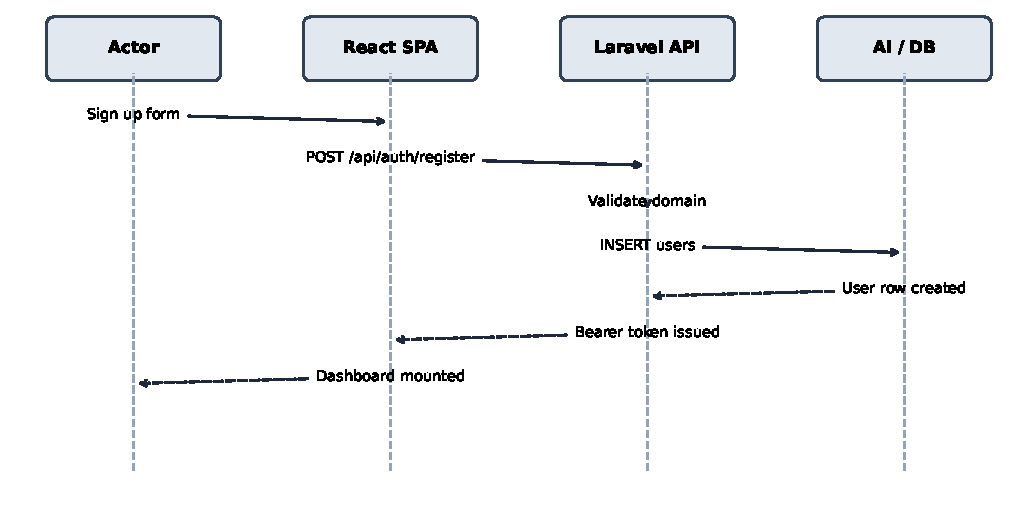
\includegraphics[width=0.75\linewidth]{figures/ssd_02.pdf}
\caption{SSD-02: Register User Sequence Diagram}
\label{fig:ssd02}
\end{figure}

\subsection{SSD-03: User Login and Token Authentication}
As shown in Figure \ref{fig:ssd03}, an existing user logs in with credentials and receives a Sanctum bearer token.

\begin{figure}[h!]
\centering
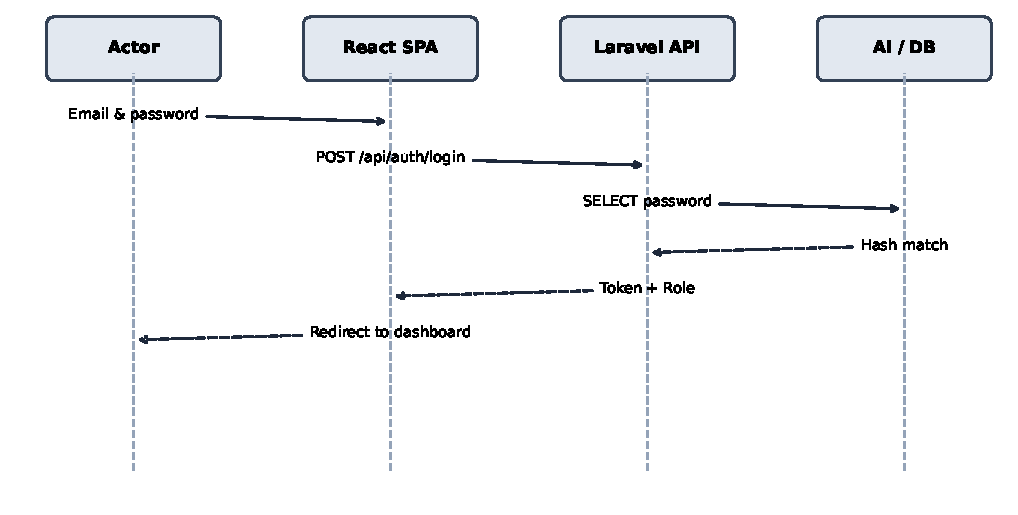
\includegraphics[width=0.75\linewidth]{figures/ssd_03.pdf}
\caption{SSD-03: User Login Sequence Diagram}
\label{fig:ssd03}
\end{figure}

\subsection{SSD-04: Create and Publish Job Vacancy}
As shown in Figure \ref{fig:ssd04}, a verified recruiter creates a job vacancy with required skills.

\begin{figure}[h!]
\centering
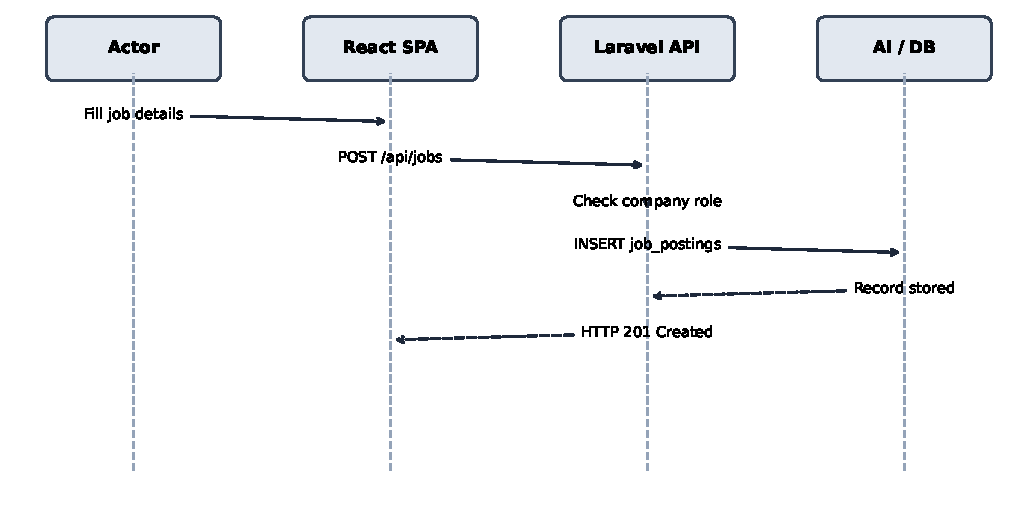
\includegraphics[width=0.75\linewidth]{figures/ssd_04.pdf}
\caption{SSD-04: Create Job Vacancy Sequence Diagram}
\label{fig:ssd04}
\end{figure}

\subsection{SSD-05: Submit Job Application and Automated AI Screening}
As shown in Figure \ref{fig:ssd05}, a candidate applies with a PDF resume, triggering synchronous AI parsing and ATS score computation.

\begin{figure}[h!]
\centering
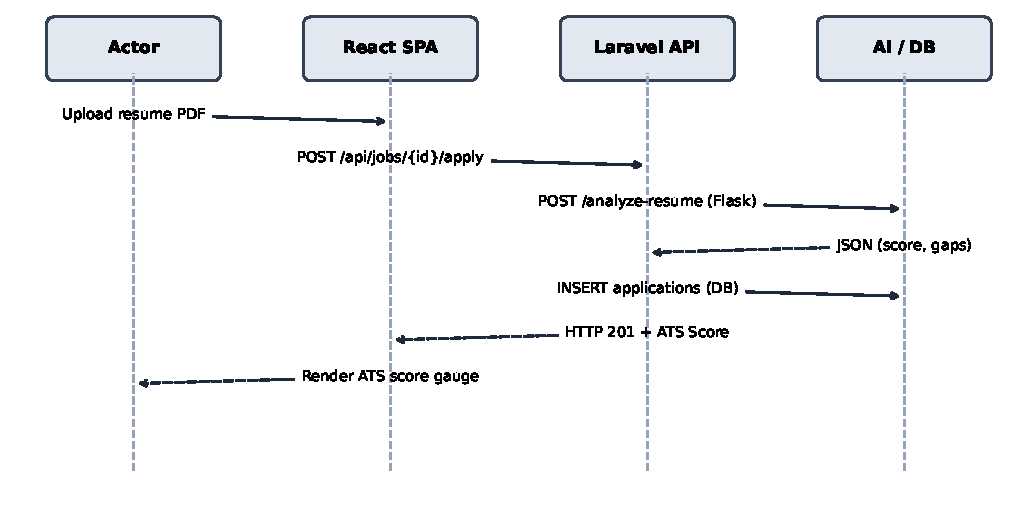
\includegraphics[width=0.85\linewidth]{figures/ssd_05.pdf}
\caption{SSD-05: Job Application and AI Screening Sequence Diagram}
\label{fig:ssd05}
\end{figure}

\subsection{SSD-06: Review AI-Ranked Candidate Shortlist}
As shown in Figure \ref{fig:ssd06}, a recruiter opens the applicant manager to review candidates ranked by ATS match percentage.

\begin{figure}[h!]
\centering
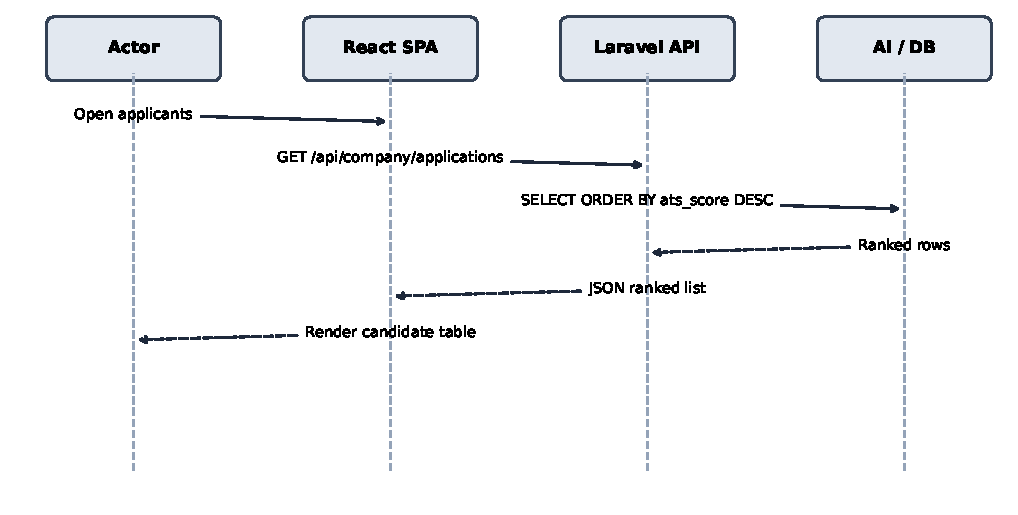
\includegraphics[width=0.75\linewidth]{figures/ssd_06.pdf}
\caption{SSD-06: Review AI-Ranked Shortlist Sequence Diagram}
\label{fig:ssd06}
\end{figure}

\subsection{SSD-07: Manage Hiring Pipeline Status}
As shown in Figure \ref{fig:ssd07}, a recruiter updates the hiring status of a candidate application.

\begin{figure}[h!]
\centering
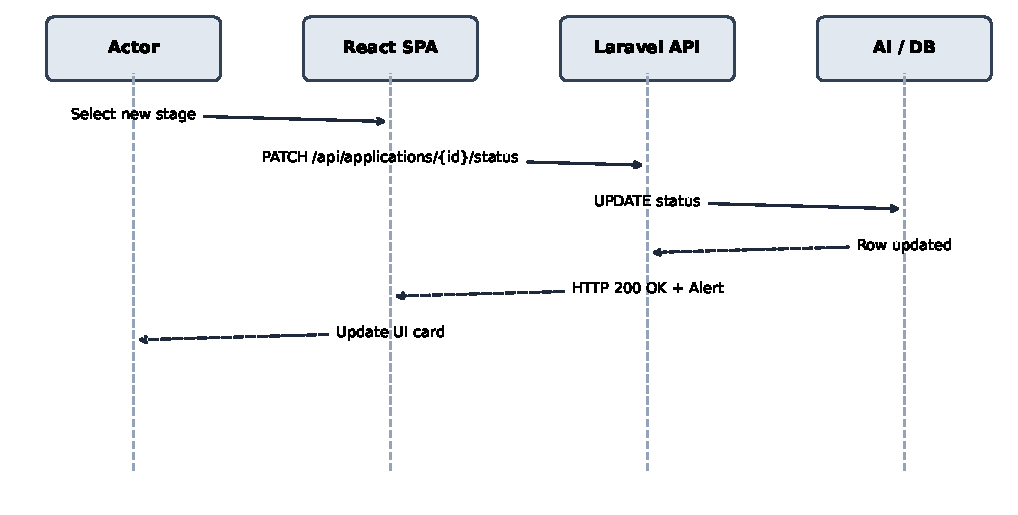
\includegraphics[width=0.75\linewidth]{figures/ssd_07.pdf}
\caption{SSD-07: Manage Hiring Pipeline Status Sequence Diagram}
\label{fig:ssd07}
\end{figure}

\subsection{SSD-08: Schedule Candidate Interview}
As shown in Figure \ref{fig:ssd08}, a recruiter schedules an interview with a candidate.

\begin{figure}[h!]
\centering
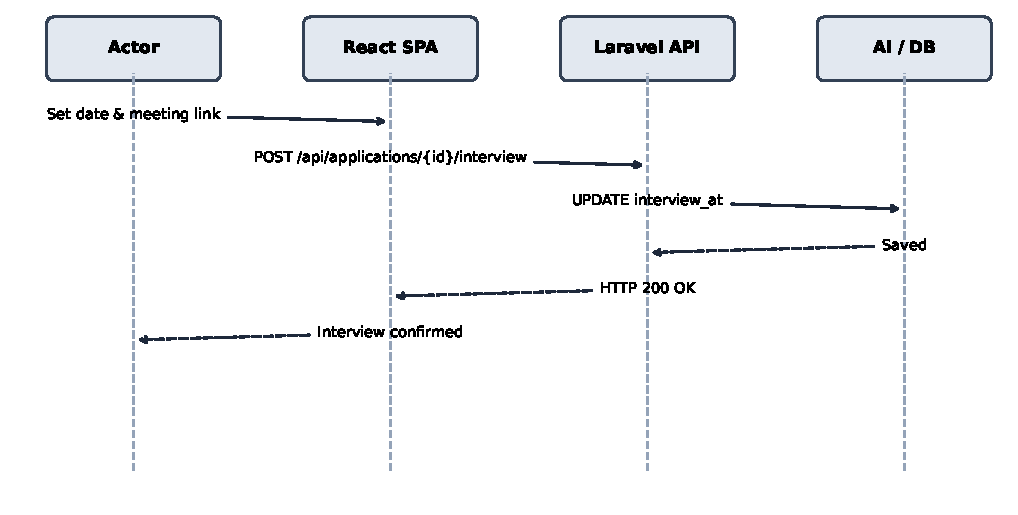
\includegraphics[width=0.75\linewidth]{figures/ssd_08.pdf}
\caption{SSD-08: Schedule Interview Sequence Diagram}
\label{fig:ssd08}
\end{figure}

\subsection{SSD-09: Real-Time In-App Messaging}
As shown in Figure \ref{fig:ssd09}, a candidate and recruiter exchange in-app messages.

\begin{figure}[h!]
\centering
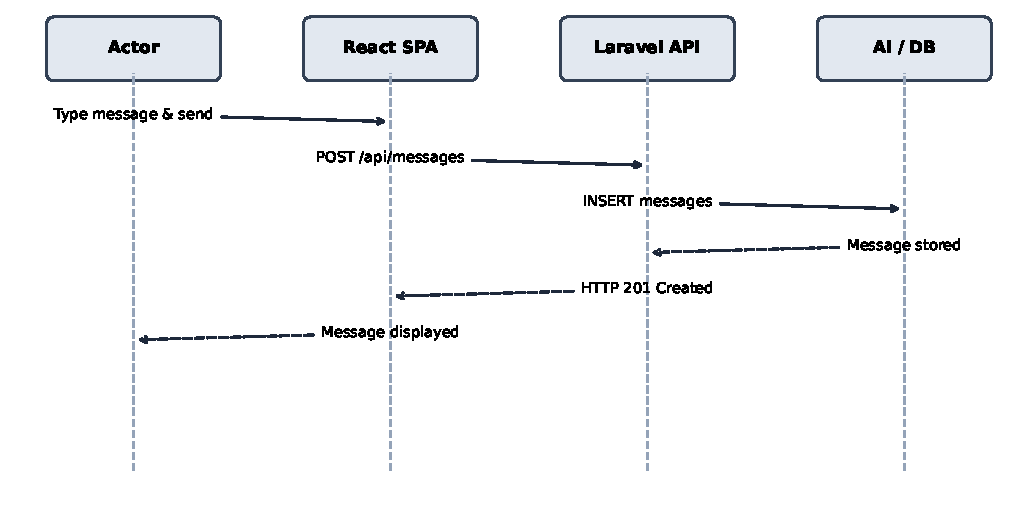
\includegraphics[width=0.75\linewidth]{figures/ssd_09.pdf}
\caption{SSD-09: In-App Messaging Sequence Diagram}
\label{fig:ssd09}
\end{figure}

\subsection{SSD-10: Verify Corporate Email Domain (Admin)}
As shown in Figure \ref{fig:ssd10}, an admin verifies a pending corporate employer domain.

\begin{figure}[h!]
\centering
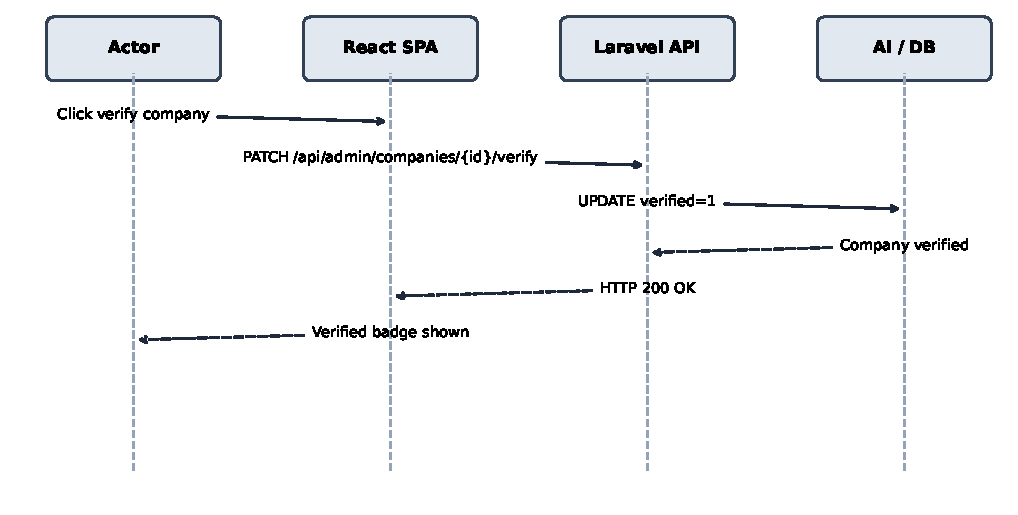
\includegraphics[width=0.75\linewidth]{figures/ssd_10.pdf}
\caption{SSD-10: Verify Corporate Domain Sequence Diagram}
\label{fig:ssd10}
\end{figure}

\section{Database Design}
The database layer of RecruitSense is built on a relational schema in MySQL 8.0 following strict third normal form (3NF) principles.

\subsection{Entity-Relationship (ER) Diagram}
Figure \ref{fig:erd_diagram} illustrates the complete Entity-Relationship diagram and cardinalities among core system entities.

\begin{figure}[h!]
\centering
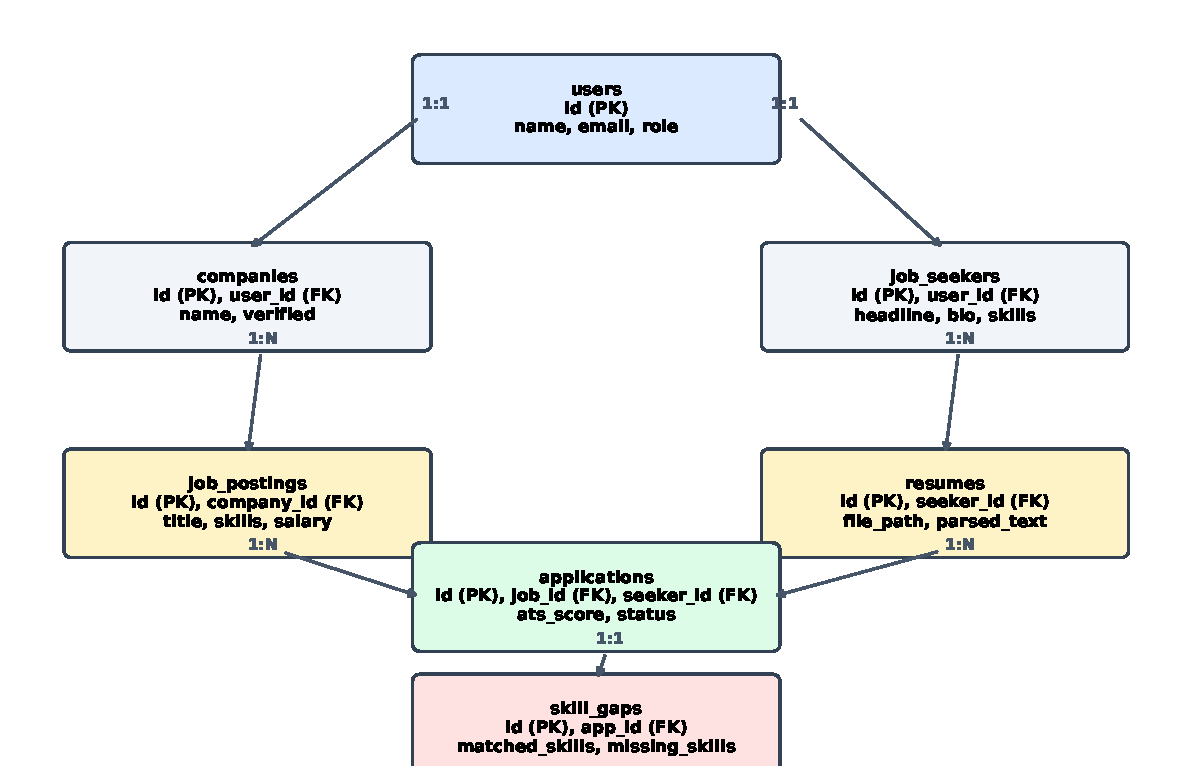
\includegraphics[width=0.85\linewidth]{figures/erd_diagram.pdf}
\caption{Entity-Relationship (ER) Diagram of RecruitSense Database Schema}
\label{fig:erd_diagram}
\end{figure}

\subsection{Complete Table Inventory}
The RecruitSense relational database consists of the following 12 core tables:
\texttt{users}, \texttt{companies}, \texttt{job\_seekers}, \texttt{job\_postings}, \texttt{resumes}, \texttt{applications}, \texttt{skill\_gaps}, \texttt{conversations}, \texttt{messages}, \texttt{notifications}, \texttt{saved\_jobs}, and \texttt{admin\_settings}.

\subsection{Core Database Schemas}

\subsubsection{Table: \texttt{users}}
\begin{table}[h!]
\centering
\small
\caption{Users Schema (\texttt{users})}
\label{tab:schema_users}
\begin{tabular}{|p{3cm}|p{2.8cm}|p{2.2cm}|p{5.5cm}|}
\hline
\textbf{Field Name} & \textbf{Type} & \textbf{Constraints} & \textbf{Description} \\ \hline
\texttt{id} & BIGINT UNSIGNED & PK, Auto-Inc & Unique user identifier \\ \hline
\texttt{name} & VARCHAR(255) & NOT NULL & Full name of user \\ \hline
\texttt{email} & VARCHAR(255) & NOT NULL, UNIQUE & Login email address \\ \hline
\texttt{password} & VARCHAR(255) & NOT NULL & Bcrypt-hashed password \\ \hline
\texttt{role} & ENUM & NOT NULL & \texttt{'job\_seeker'}, \texttt{'company'}, \texttt{'admin'} \\ \hline
\texttt{status} & VARCHAR(50) & Default: 'active' & Account state: active, suspended \\ \hline
\texttt{created\_at} & TIMESTAMP & NULL & Creation timestamp \\ \hline
\end{tabular}
\end{table}

\subsubsection{Table: \texttt{companies}}
\begin{table}[h!]
\centering
\small
\caption{Companies Schema (\texttt{companies})}
\label{tab:schema_companies}
\begin{tabular}{|p{3cm}|p{2.8cm}|p{2.2cm}|p{5.5cm}|}
\hline
\textbf{Field Name} & \textbf{Type} & \textbf{Constraints} & \textbf{Description} \\ \hline
\texttt{id} & BIGINT UNSIGNED & PK, Auto-Inc & Unique company identifier \\ \hline
\texttt{user\_id} & BIGINT UNSIGNED & FK \texttt{users.id} & Reference to owner user \\ \hline
\texttt{company\_name} & VARCHAR(255) & NOT NULL & Corporate name \\ \hline
\texttt{website} & VARCHAR(255) & NULL & Corporate website \\ \hline
\texttt{verified} & BOOLEAN & Default: 0 & Domain verification flag \\ \hline
\texttt{created\_at} & TIMESTAMP & NULL & Creation timestamp \\ \hline
\end{tabular}
\end{table}

\subsubsection{Table: \texttt{job\_postings}}
\begin{table}[h!]
\centering
\small
\caption{Job Postings Schema (\texttt{job\_postings})}
\label{tab:schema_job_postings}
\begin{tabular}{|p{3cm}|p{2.8cm}|p{2.2cm}|p{5.5cm}|}
\hline
\textbf{Field Name} & \textbf{Type} & \textbf{Constraints} & \textbf{Description} \\ \hline
\texttt{id} & BIGINT UNSIGNED & PK, Auto-Inc & Unique job vacancy ID \\ \hline
\texttt{company\_id} & BIGINT UNSIGNED & FK \texttt{companies.id} & Reference to hiring company \\ \hline
\texttt{title} & VARCHAR(255) & NOT NULL & Vacancy title \\ \hline
\texttt{description} & TEXT & NOT NULL & Job responsibilities and requirements \\ \hline
\texttt{required\_skills}& TEXT & NOT NULL & Comma-separated required skills \\ \hline
\texttt{salary\_min} & DECIMAL(10,2) & NULL & Minimum compensation \\ \hline
\texttt{salary\_max} & DECIMAL(10,2) & NULL & Maximum compensation \\ \hline
\texttt{status} & VARCHAR(50) & Default: 'active' & \texttt{'active'}, \texttt{'draft'}, \texttt{'closed'} \\ \hline
\end{tabular}
\end{table}

\subsubsection{Table: \texttt{applications}}
\begin{table}[h!]
\centering
\small
\caption{Applications Schema (\texttt{applications})}
\label{tab:schema_applications}
\begin{tabular}{|p{3cm}|p{2.8cm}|p{2.2cm}|p{5.5cm}|}
\hline
\textbf{Field Name} & \textbf{Type} & \textbf{Constraints} & \textbf{Description} \\ \hline
\texttt{id} & BIGINT UNSIGNED & PK, Auto-Inc & Unique application ID \\ \hline
\texttt{job\_posting\_id}& BIGINT UNSIGNED & FK \texttt{job\_postings.id}& Reference to target vacancy \\ \hline
\texttt{job\_seeker\_id} & BIGINT UNSIGNED & FK \texttt{job\_seekers.id} & Reference to candidate \\ \hline
\texttt{resume\_path} & VARCHAR(255) & NOT NULL & Obfuscated file path on disk \\ \hline
\texttt{ats\_score} & DECIMAL(5,2) & NOT NULL & Computed overall ATS match \% \\ \hline
\texttt{status} & VARCHAR(50) & Default: 'applied' & \texttt{'applied'}, \texttt{'screening'}, \texttt{'shortlisted'}, \dots \\ \hline
\texttt{interview\_at} & DATETIME & NULL & Scheduled interview timestamp \\ \hline
\end{tabular}
\end{table}

\subsubsection{Table: \texttt{skill\_gaps}}
\begin{table}[h!]
\centering
\small
\caption{Skill Gaps Schema (\texttt{skill\_gaps})}
\label{tab:schema_skill_gaps}
\begin{tabular}{|p{3cm}|p{2.8cm}|p{2.2cm}|p{5.5cm}|}
\hline
\textbf{Field Name} & \textbf{Type} & \textbf{Constraints} & \textbf{Description} \\ \hline
\texttt{id} & BIGINT UNSIGNED & PK, Auto-Inc & Unique skill gap ID \\ \hline
\texttt{application\_id} & BIGINT UNSIGNED & FK \texttt{applications.id}& Reference to application \\ \hline
\texttt{matched\_skills} & JSON & NOT NULL & Array of matched skill strings \\ \hline
\texttt{missing\_skills} & JSON & NOT NULL & Array of missing skill strings \\ \hline
\texttt{bonus\_skills} & JSON & NULL & Array of extra recognized skills \\ \hline
\end{tabular}
\end{table}

\section{Graphical User Interface (GUI) Design}
The user interface of RecruitSense is engineered for operational speed, accessibility, and visual clarity using Tailwind CSS design tokens.

\subsection{Job Seeker GUI Direction}
\begin{itemize}
    \item \textbf{Job Discovery Portal:} Live keyword search bar, category chips, salary range sliders, and dynamic job cards displaying verified employer badges.
    \item \textbf{Interactive Application Modal:} Single-click resume file uploader supporting drag-and-drop PDF ingestion with progress bars.
    \item \textbf{ATS Score Visualizer:} Instant diagnostic modal rendering overall match percentage gauge, green badges for matched skills, and red badges for missing skill gaps.
\end{itemize}

\subsection{Recruiter GUI Direction}
\begin{itemize}
    \item \textbf{Job Posting Builder:} Structured form with auto-tokenizing skill input tags, salary bounds, and requirement validation.
    \item \textbf{Applicant Ranking Console:} Tabular view of all candidates sorted automatically by computed ATS score, complete with quick-action status dropdowns and resume viewers.
    \item \textbf{Hiring Pipeline Board:} Kanban-style or status-filtered interface to move candidates across review, interview, and offer stages.
\end{itemize}

\subsection{Admin GUI Direction}
\begin{itemize}
    \item \textbf{Company Verification Queue:} Review pending employer registrations and corporate domain authenticity.
    \item \textbf{Analytics Dashboard:} Graphical visualizations of platform adoption, parsed resumes, and ATS score distributions.
\end{itemize}

\section{External Interfaces and Deployment Pipeline}
Figure \ref{fig:cicd_pipeline} illustrates the Continuous Integration and Deployment (CI/CD) and service interface model of RecruitSense.

\begin{figure}[h!]
\centering
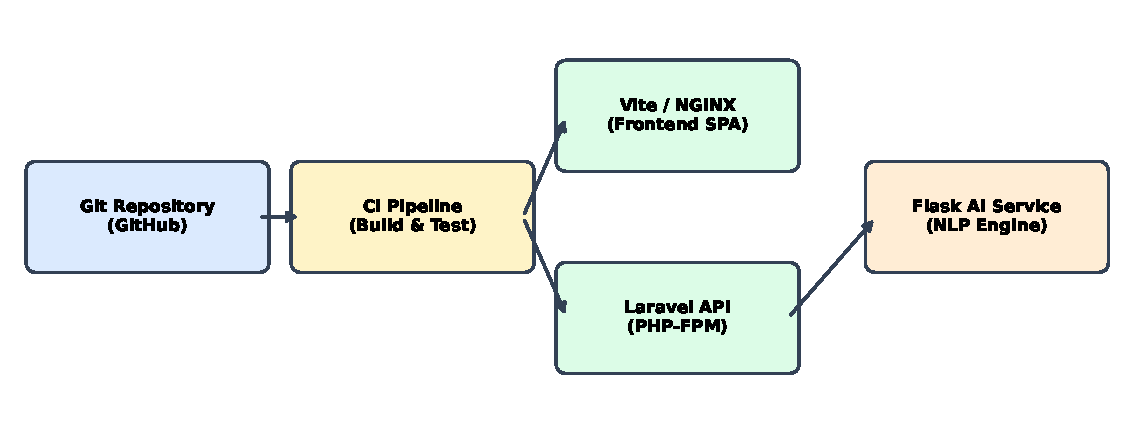
\includegraphics[width=0.8\linewidth]{figures/cicd_pipeline.pdf}
\caption{CI/CD and Service Deployment Pipeline of RecruitSense}
\label{fig:cicd_pipeline}
\end{figure}

\section{Chapter Summary}
This chapter presented the complete system design of \textbf{RecruitSense}. It articulated the 4-tier decoupled architecture, analyzed design constraints and assumptions, presented the state-machine methodology and high-level block models, detailed 10 System Sequence Diagrams (SSDs) covering core workflows, documented the 3NF MySQL relational database schema and data dictionaries, and established GUI directions and CI/CD deployment pipelines. This design provides the structural blueprint for the technical realization presented in Chapter \ref{chap:sysImplementation}.
